\documentclass{beamer}
\usetheme{BauhausNeuralFEM} 
\usepackage{amssymb}


% --- Title info ---
\title[Post-processing \& Error Norms]{From FEM to Neural Operators: Scientific Machine Learning for Computational Mechanics\\[0.4cm]}
\subtitle{Post-processing and Error Norms}
\author{Dr-Ing Jorge Alberto L\'{o}pez Zerme\~{n}o}
\date{}

\graphicspath {{Figures/}}

% --- Helpful macros ---
\newcommand{\R}{\mathbb{R}}
\newcommand{\bK}{\mathbf{K}}
\newcommand{\bU}{\mathbf{U}}
\newcommand{\bfvec}{\mathbf{f}}
\newcommand{\be}{\mathbf{e}}
\newcommand{\domain}{\Omega}
\newcommand{\boundary}{\Gamma}
\newcommand{\diri}{\Gamma_D}
\newcommand{\neum}{\Gamma_N}

\begin{document}
	
	{
		\usebackgroundtemplate{
			\begin{tikzpicture}[remember picture,overlay]
				\node[opacity=0.25,inner sep=0pt] at (current page.center)
				{
\includegraphics[width=\paperwidth,height=\paperheight]{Background.pdf}};
			\end{tikzpicture}
		}
		\begin{frame}[plain]
			\centering
			\begin{minipage}{0.21\textwidth}
				\centering
				
\includegraphics[width=\linewidth]{Bauhaus_Logo.png}
			\end{minipage}\hspace{105pt}
			\begin{minipage}{0.3\textwidth}
				\centering
				
\includegraphics[width=\linewidth]{JHU_Logo.png}
			\end{minipage}
			
			\titlepage
			\vspace{-35pt}
			Bauhaus Spring School 2026
			
		\end{frame}
	}
	
	%====================
	\begin{frame}{What we already have}
		\normalsize
		\textbf{Solution fields:}
		
		\begin{minipage}{0.4\textwidth}
			\begin{center}
				\footnotesize
				\textbf{1D:}
			\end{center}
		\end{minipage}\hfill
		\begin{minipage}{0.1\textwidth}
			
		\end{minipage}
		\begin{minipage}{0.4\textwidth}
			\begin{center}
				\footnotesize
				\textbf{2D:}
			\end{center}
		\end{minipage}
		
		\begin{minipage}{0.4\textwidth}
			\begin{center}
				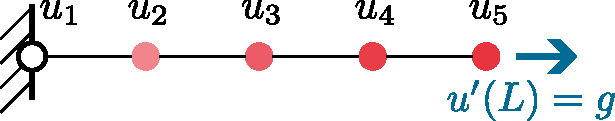
\includegraphics[width=\linewidth]{Solution_1D.pdf}
			\end{center}
		\end{minipage}\hfill
		\begin{minipage}{0.1\textwidth}
			\begin{center}
				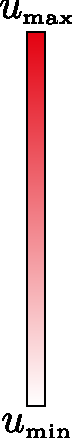
\includegraphics[width=0.6\linewidth]{u_Colorbar.pdf}
			\end{center}
		\end{minipage}\hfill
		\begin{minipage}{0.4\textwidth}
			\begin{center}
				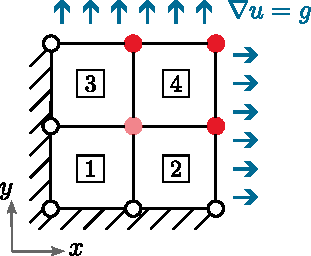
\includegraphics[width=0.9\linewidth]{Solution_2D.pdf}
			\end{center}
		\end{minipage}
		
		\vspace{6pt}
		\small
		\begin{itemize}
			\item Nodal solution values $\mathbf{U}$ obtained from the FEM discretization.
			\item Next step: Computing $u$ and $u'$ at any point, and error norms.
		\end{itemize}
	\end{frame}
	
	%====================
	\begin{frame}{Interpolation of $u$ and $u'$}
		\begin{minipage}{0.48\textwidth}
			\begin{center}
				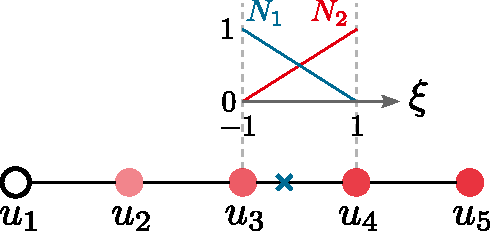
\includegraphics[width=0.9\linewidth]{u_Interpolation.pdf}
			\end{center}
		\end{minipage}\hfill
		\begin{minipage}{0.48\textwidth}
			\small
			\vspace{45pt}
			\begin{equation*}
				u(x(\xi)) = \sum_i N_i(\xi)\,u_i
			\end{equation*}
		\end{minipage}
		
		\vspace{25pt}
		\begin{minipage}{0.48\textwidth}
			\begin{center}
				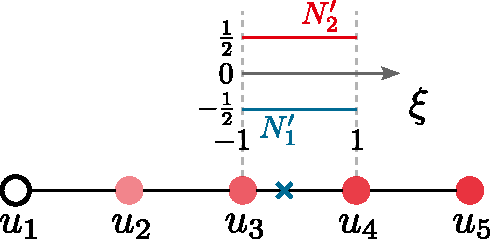
\includegraphics[width=0.9\linewidth]{du_Interpolation.pdf}
			\end{center}
		\end{minipage}\hfill
		\begin{minipage}{0.48\textwidth}
			\small
			\vspace{45pt}
			\begin{equation*}
				u'(x(\xi)) = \sum_i N'_i(\xi\,)u_i
			\end{equation*}
		\end{minipage}
	\end{frame}
	
	%====================
	\begin{frame}{Error field and norms}
		\begin{minipage}{0.48\textwidth}
			\normalsize
			\textbf{$L^2$-norm:}
			
			\footnotesize
			\[
			\|e\|_{L^2(\domain)}
			= \left(
			\int_0^L \big(u(x) - u_h(x)\big)^2 \, dx
			\right)^{1/2}
			\]
		\end{minipage}\hfill
		\begin{minipage}{0.48\textwidth}
			\begin{center}
				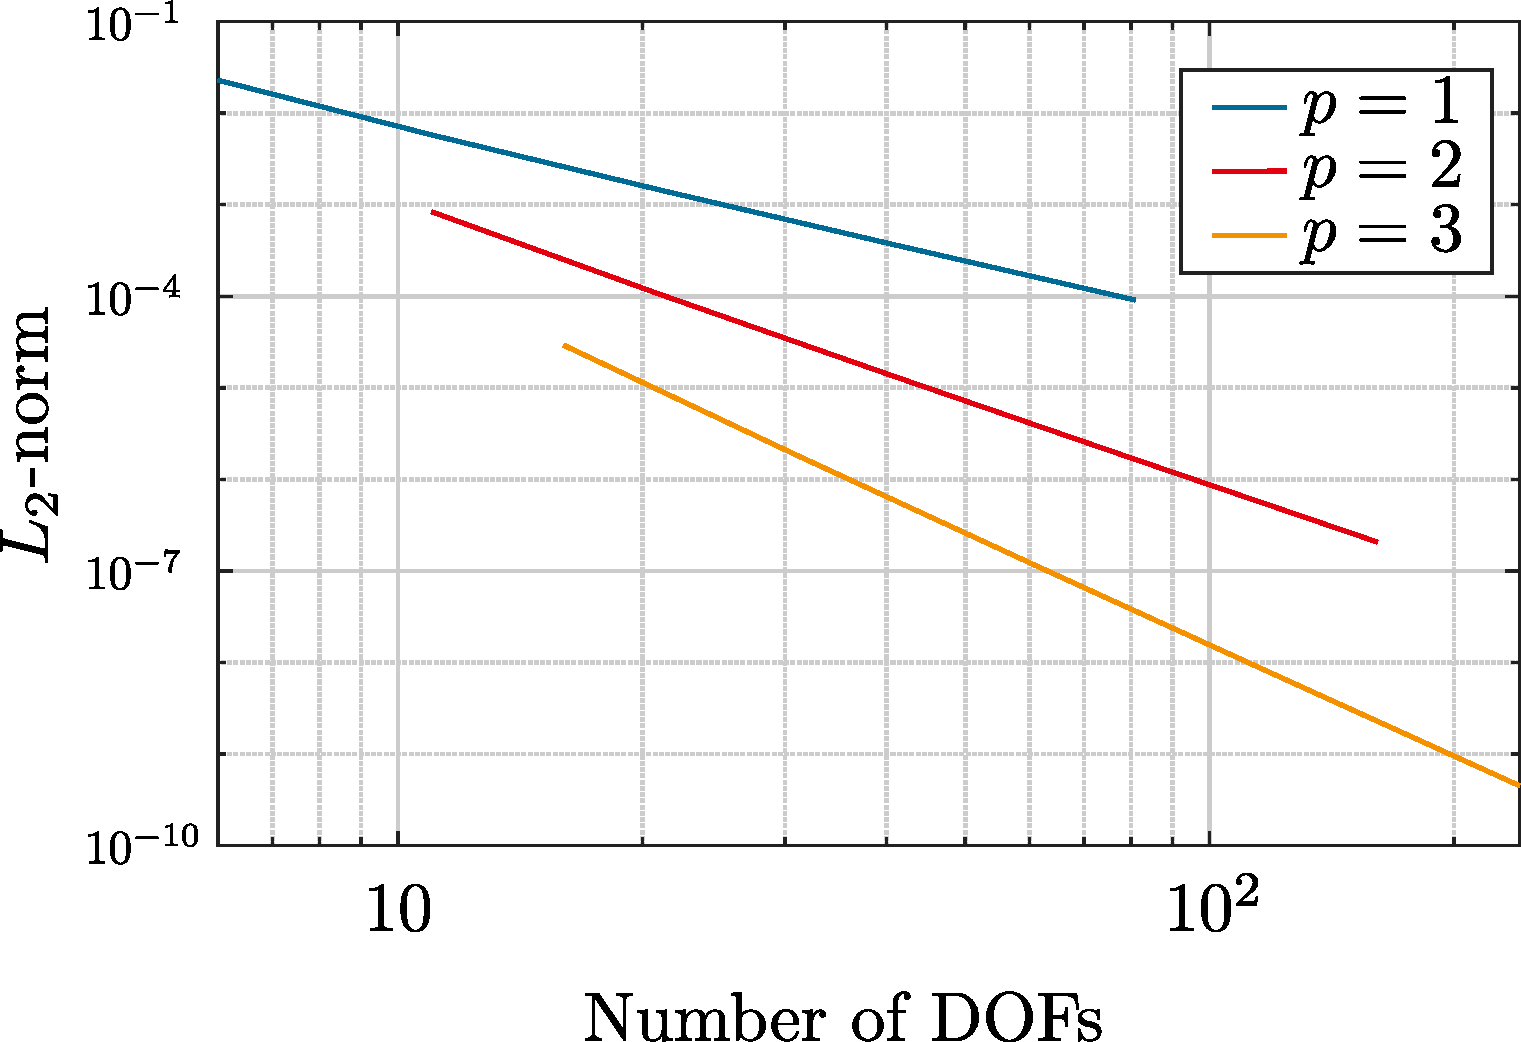
\includegraphics[width=0.95\linewidth]{Figure_L2_Norm.pdf}
			\end{center}
		\end{minipage}
		
		\vspace{25pt}
		\begin{minipage}{0.48\textwidth}
			\normalsize
			\textbf{Energy-norm:}
			
			\footnotesize
			\[
			\|e\|_E
			= \left(
			\int_0^L k(x)\,\big(u'(x) - u'_h(x)\big)^2 \, dx
			\right)^{1/2}
			\]
		\end{minipage}\hfill
		\begin{minipage}{0.48\textwidth}
			\begin{center}
				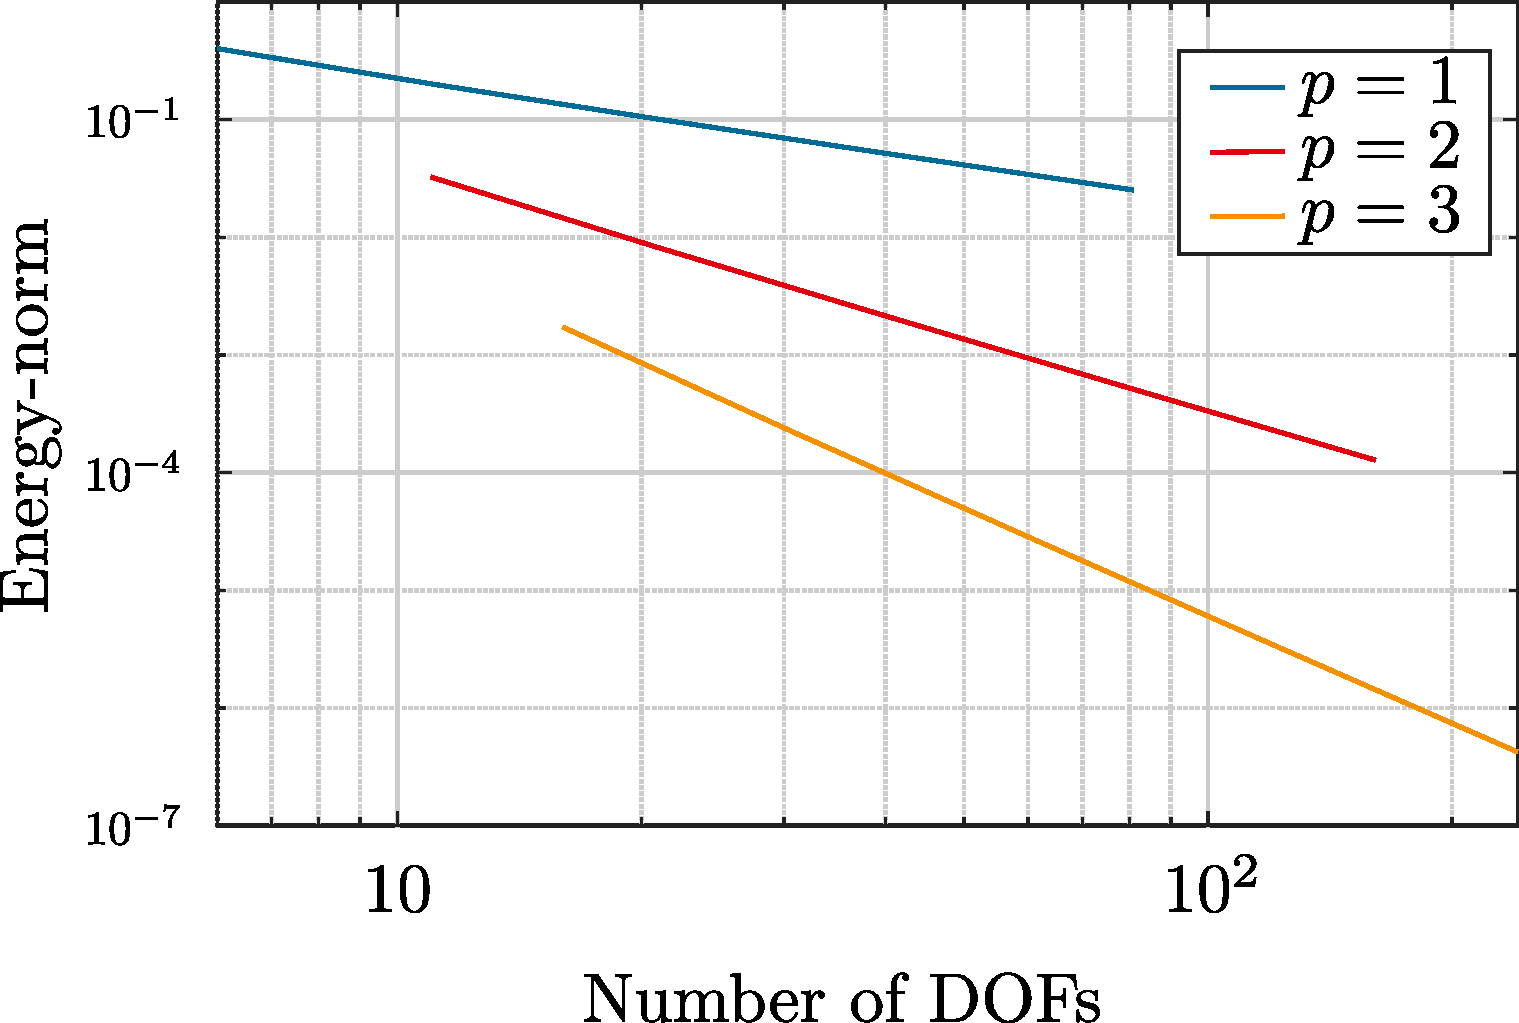
\includegraphics[width=0.95\linewidth]{Figure_Energy_Norm.pdf}
			\end{center}
		\end{minipage}
	\end{frame}
	

	
	%====================
	\begin{frame}{Conclusions and outlook}
			\small
			\textbf{Conclusions}
			\footnotesize
			\begin{itemize}
				\item Post-processing uses the same tools as assembly:
				
				\begin{itemize}
					\item[-] \footnotesize Shape functions, gradients, Jacobians, quadrature.
				\end{itemize}
				\item We can reconstruct $u(x)$ and $u'(x)$ at any point.
				\item $L^2$- and energy-norms quantify the error in $u$ and $\nabla u$.
			\end{itemize}
			
			\vspace{4pt}
			\small
			\textbf{Outlook (PINNs and Neural Operators)}
			\footnotesize
			\begin{itemize}
				\item PINNs: PDE residuals and boundary conditions appear in the loss;
				error norms can be used for validation.
				\item Neural Operators: often trained on FEM solution fields
				(and compared using similar error norms).
			\end{itemize}
	\end{frame}
	
\end{document}
